\documentclass[aspectratio=169]{beamer}

% ============================================================
% Theme & Colors
% ============================================================
\usetheme{Madrid}
\usecolortheme{default}

\definecolor{darkgray}{RGB}{40,42,54}
\definecolor{midgray}{RGB}{120,120,120}
\definecolor{lightbg}{RGB}{245,245,247}
\definecolor{softbg}{RGB}{250,250,252}
\definecolor{highlight}{RGB}{0,102,204}
\definecolor{accentred}{RGB}{180,30,30}
\definecolor{accentgreen}{RGB}{30,130,60}
\definecolor{accentamber}{RGB}{200,140,20}

\setbeamercolor{title}{fg=white}
\setbeamercolor{subtitle}{fg=white}
\setbeamercolor{author}{fg=white}
\setbeamercolor{frametitle}{bg=darkgray, fg=white}
\setbeamercolor{structure}{fg=darkgray}
\setbeamercolor{block title}{bg=darkgray, fg=white}
\setbeamercolor{block body}{bg=lightbg, fg=darkgray}
\setbeamercolor{alerted text}{fg=accentred}
\setbeamercolor{itemize item}{fg=darkgray}
\setbeamercolor{itemize subitem}{fg=midgray}
\setbeamerfont{frametitle}{size=\Large, series=\bfseries}
\setbeamerfont{block title}{size=\small, series=\bfseries}
\setbeamertemplate{navigation symbols}{}
\setbeamertemplate{footline}[frame number]
\setbeamertemplate{itemize item}[circle]
\setbeamertemplate{itemize subitem}[triangle]

% ============================================================
% Packages
% ============================================================
\usepackage[utf8]{inputenc}
\usepackage[T1]{fontenc}
\usepackage[spanish]{babel}
\usepackage{booktabs}
\usepackage{multirow}
\usepackage{colortbl}
\usepackage{xcolor}
\usepackage{graphicx}
\usepackage{tikz}
\usetikzlibrary{positioning, arrows.meta, shapes.geometric, fit, backgrounds}
\usepackage[absolute,overlay]{textpos}

% Custom commands
\newcommand{\hl}[1]{\textcolor{highlight}{\textbf{#1}}}
\newcommand{\good}[1]{\textcolor{accentgreen}{#1}}
\newcommand{\bad}[1]{\textcolor{accentred}{#1}}

% ============================================================
% Title
% ============================================================
\title[Clasificación multimodal robusta]{Clasificación multimodal de esperanza de vida\\\large con robustez ante datos faltantes}
\subtitle{ARA}
\author[Gómez \& Pacheco]{Andrés Pacheco Millán \and Miquel Gómez Corral}
\institute[UPV]{Máster en Inteligencia Artificial,
           Reconocimiento de Formas e Imagen Digital\\
           Universitat Politècnica de València}
\date{}

% ============================================================
\begin{document}

\begin{frame}[plain]
  \titlepage
  \begin{tikzpicture}[remember picture, overlay]
    \node[anchor=south east, font=\small] at ([xshift=-1.2cm, yshift=0.6cm]current page.south east)
      {Miquel Gómez Corral $\cdot$ Andrés Pacheco Millán};
  \end{tikzpicture}
\end{frame}

% ============================================================
\begin{frame}{Índice}
  \begin{columns}[T]
    \begin{column}{0.48\textwidth}
      \begin{enumerate}
        \item Introducción y motivación
        \item Trabajo relacionado
        \item Descripción de la tarea
        \item Dataset
        \item Arquitectura del modelo
      \end{enumerate}
    \end{column}
    \begin{column}{0.48\textwidth}
      \begin{enumerate}\setcounter{enumi}{5}
        \item Nuestras contribuciones
        \item Diseño experimental
        \item Resultados
        \item Conclusiones y trabajo futuro
      \end{enumerate}
    \end{column}
  \end{columns}
\end{frame}

% ============================================================
\section{Introducción y motivación}

\begin{frame}{Introducción y motivación}
    En la práctica clínica \hl{rara vez se dispone de todos los datos} de un paciente al momento de decidir.

    \medskip
    \textbf{¿Por qué faltan datos?}
    \begin{itemize}
      \item Urgencia o coste: no siempre hay tiempo o recursos para todas las secuencias MRI
      \item Fallos técnicos o paciente no colaborador
      \item Registros incompletos o perdidos
    \end{itemize}

    \medskip
    \begin{block}{Objetivo}
      Predecir la esperanza de vida en glioblastoma con un modelo \hl{robusto ante datos faltantes}.
    \end{block}
\end{frame}

% ============================================================
\section{Dataset}

\begin{frame}{Dataset UPenn-GBM}
  \begin{columns}[T]
    \begin{column}{0.50\textwidth}
      \centering\footnotesize
      \begin{tabular}{lr}
        \toprule
        \textbf{Variable} & \textbf{Valor} \\
        \midrule
        Pacientes / muestras    & 603 / 630 \\
        Edad media              & 62.7 $\pm$ 12.5 años \\
        Género (M\,/\,F)        & 378 / 252 \\
        Supervivencia media     & 496 días \\
        \midrule
        \rowcolor{lightbg}
        \textbf{Clase 0 ($\leq$12m)} & \textbf{305} \\
        \rowcolor{lightbg}
        \textbf{Clase 1 ($>$12m)}    & \textbf{339} \\
        \bottomrule
      \end{tabular}

      \vspace{0.8em}
      \begin{tabular}{lrr}
        \toprule
        \textbf{Split} & \textbf{Pacientes} & \textbf{\%} \\
        \midrule
        Entrenamiento & 482 & 80\% \\
        Validación    &  60 & 10\% \\
        Test          &  61 & 10\% \\
        \bottomrule
      \end{tabular}
    \end{column}
    \begin{column}{0.46\textwidth}
      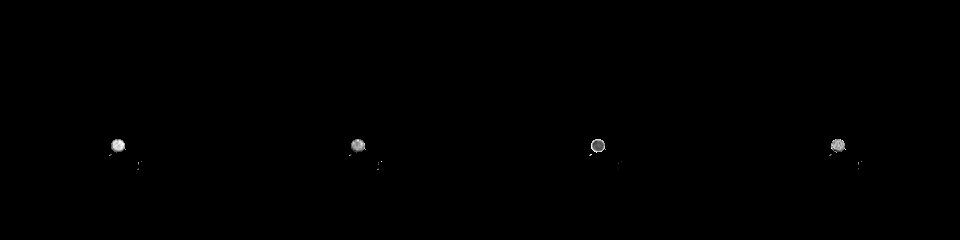
\includegraphics[width=\textwidth]{images/UPENN-GBM-00465.png}

      \begin{block}{MRI 3D multimodal glioblastoma}
        \small
        \textbf{T1}: anatomía estructural sana \\
        \textbf{T1ce}: tumor activo (realce de contraste) \\
        \textbf{T2}: contenido de agua / líquido \\
        \textbf{FLAIR}: edema peritumoral \\
        \textbf{Tabulares}: Datos clínicos \\
        \textbf{Radiómicos}: Características extraídas de la imagen
      \end{block}
    \end{column}
  \end{columns}
\end{frame}


% ============================================================
\section{Descripción de la tarea}

\begin{frame}{Descripción de la tarea}
      \textbf{Clasificación binaria de supervivencia}
      \begin{itemize}
        \item \hl{Clase 1} --- supervivencia $>$ 12 meses
        \item \hl{Clase 0} --- supervivencia $\leq$ 12 meses
      \end{itemize}

      \medskip
      \textbf{Tres modalidades de entrada}
      \begin{itemize}
        \item \textbf{MRI 3D}: 4 secuencias (T1, T1Gd, T2, FLAIR)
        \item \textbf{Clínicos}: edad, género, KPS, IDH1, MGMT, GTR
        \item \textbf{Radiómicos}: 144 \textit{features} por región (ED, ET, NC)
      \end{itemize}

      \medskip
      \begin{block}{El reto central}
        \small En inferencia, \textbf{cualquier combinación de estas entradas puede estar ausente}. El modelo debe funcionar bien en todos los casos, sin lógica condicional codificada a mano.
      \end{block}
\end{frame}

% ============================================================
\section{Trabajo relacionado}

\begin{frame}{Trabajo relacionado}
  \begin{columns}[T]
    \begin{column}{0.52\textwidth}
      \textbf{Gomaa et al.\ (2024)}\\
      \textit{\small Comprehensive multimodal deep learning survival prediction enabled by a transformer architecture}

      \medskip
  \begin{itemize}
    \item Dos vistas con \textit{cutout} y \textit{patch-swapping}
    \item Pretraining auto-supervisado:
    \begin{itemize}
      \item \textit{Contrastive Learning}: ambas representaciones similares entre sí
      \item \textit{Context Reconstruction}: capacidad de reconstruir la imagen original
    \end{itemize}
    \item \hl{Cross-attention} entre características fisiológicas y características extraídas del ViT
  \end{itemize}

  \medskip
  \textbf{Punto de partida}: tomamos esta arquitectura y la extendemos para \hl{tolerar datos faltantes} e incorporar radiómicos como nueva modalidad.
    \end{column}
    \begin{column}{0.4\textwidth}
      \centering
      \fbox{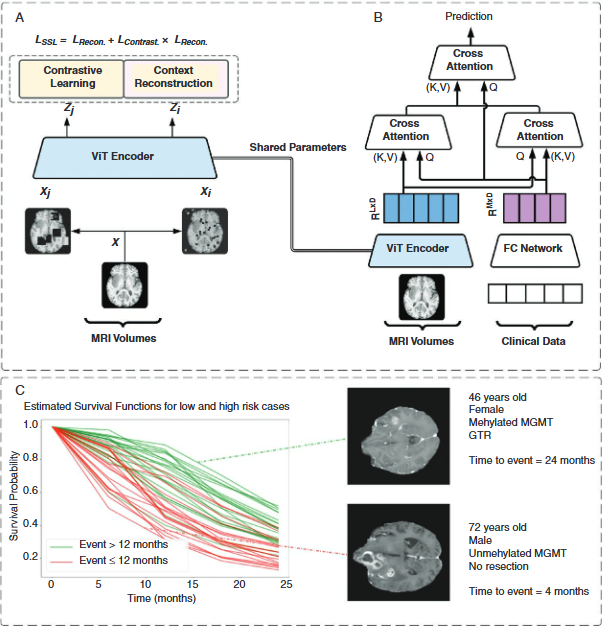
\includegraphics[width=\textwidth]{images/gomaa_architecture.png}}
      \vspace{0.2em}
      {\scriptsize\textit{Arquitectura original de Gomaa et al.\ (2024).}}
    \end{column}
  \end{columns}
\end{frame}



% ============================================================
\begin{frame}{Arquitectura — Propuesta inicial}
  \begin{columns}[T]
    \begin{column}{0.50\textwidth}
      \small
      \textbf{Fusión vía Cross-Attention}
      \begin{itemize}
        \item Radiómicos atienden a características del ViT
      \end{itemize}

      \medskip
      \textbf{\color{red}Limitaciones}
      \begin{itemize}
        \item Radiómicos extraídos \textbf{de la segmentación}: información redundante con la imagen MRI
        \item Sin imagen, el cross-attention \textbf{no tiene tokens} a los que atender $\to$ el módulo colapsa
        \item La fusión no distingue si una modalidad \textbf{falta o está presente}
      \end{itemize}
    \end{column}
    \begin{column}{0.46\textwidth}
      \centering
      \fbox{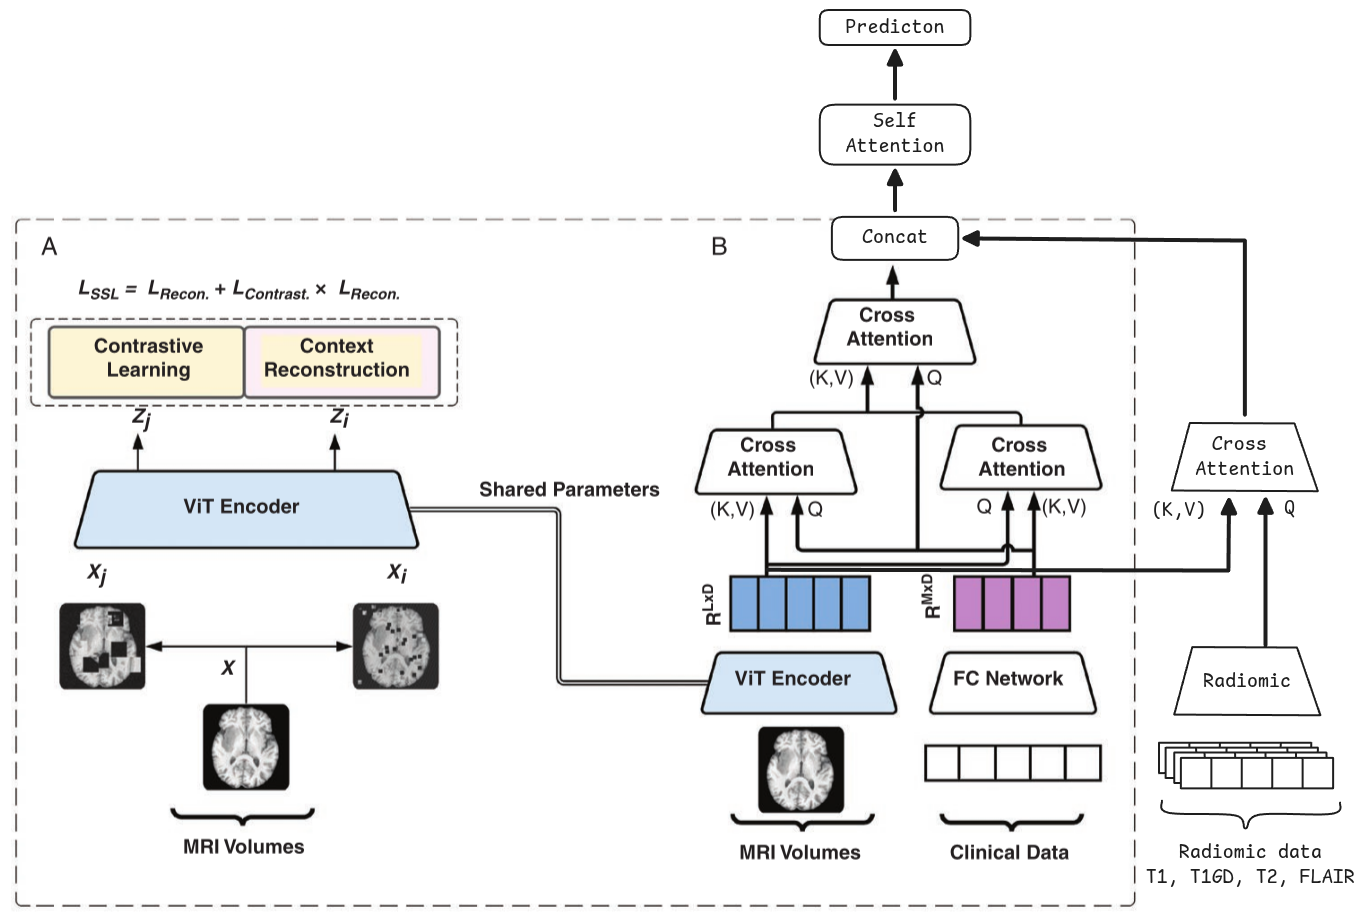
\includegraphics[width=\textwidth]{images/init.png}}
      \vspace{0.3em}
      {\scriptsize\textit{Cross-attention entre imagen (azul) y clínicos (morado).}}
    \end{column}
  \end{columns}
\end{frame}


\begin{frame}{Arquitectura — Gated Fusion}
  \begin{columns}[T]
    \begin{column}{0.50\textwidth}
      \small
      \textbf{Puerta lógica por dimensión}
      \begin{itemize}
        \item Sigmoid \textbf{por dimensión}: cada canal aprende a incluirse o excluirse
        \item Si falta alguna modalidad, el gate aprende a \textbf{anularla}
      \end{itemize}

      \small
      \[
        \mathbf{h} = (1-\sigma)\odot\mathbf{r} + \sigma\odot\mathbf{v}
      \]

      \vspace{0.1em}
      \textbf{\color{teal}Ventajas}
      \begin{itemize}
        \item Tolera ausencia de modalidades sin degradar el pipeline
        \item El gate aprende a ignorar redundancia imagen-radiómicos
        \item Añade modalidad nueva sin romper la arquitectura base
      \end{itemize}
    \end{column}
    \begin{column}{0.46\textwidth}
      \centering
      \fbox{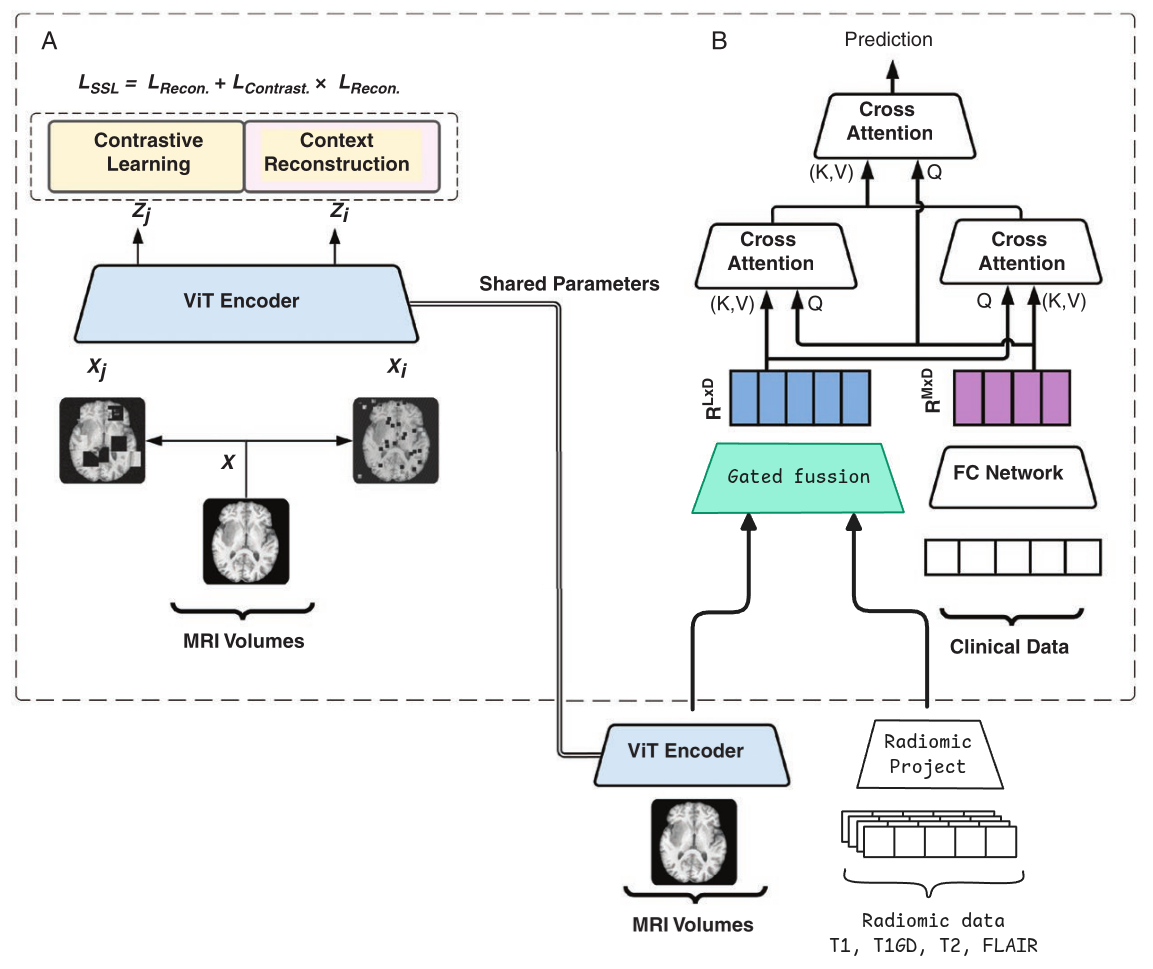
\includegraphics[width=\textwidth]{images/final.png}}
      % \vspace{0.3em}
      {\scriptsize\textit{Gated Fusion (verde) integra radiómicos antes del cross-attention.}}
    \end{column}
  \end{columns}
\end{frame}

% ============================================================
\section{Nuestras contribuciones}

\begin{frame}{Nuestras contribuciones}
  \begin{columns}[T]
    \begin{column}{0.48\textwidth}
      \textbf{Robustez ante datos faltantes}
      \begin{itemize}
        \item \hl{Data dropout}: simulación sistemática de ausencias durante el entrenamiento
        \item El modelo aprende a funcionar con \textbf{cualquier combinación} de modalidades
      \end{itemize}

      \medskip
      \textbf{Nueva modalidad: radiómicos}
      \begin{itemize}
        \item Gestionados por un \hl{sigmoid gate}: el modelo decide cuándo y cuánto usarlos
        \item Si la modalidad falta, el gate la anula automáticamente
      \end{itemize}
    \end{column}
    \begin{column}{0.48\textwidth}

      \medskip
      \begin{exampleblock}{Resultado}
        \small El modelo acepta \textbf{cualquier combinación de entradas} en inferencia, sin necesidad de reentrenar.
      \end{exampleblock}
    \end{column}
  \end{columns}
\end{frame}
% ============================================================
\begin{frame}{Dataset Extra: BraTS 2021}
  \begin{columns}[T]
    \begin{column}{0.50\textwidth}
      \centering\footnotesize
      \begin{tabular}{lr}
        \toprule
        \textbf{Variable} & \textbf{Valor} \\
        \midrule
        Pacientes              & 1251 \\
        Secuencias MRI         & 4 (T1, T1ce, T2, FLAIR) \\
        Preprocesado           & Co-registrado, sin cráneo \\
        Segmentación           & Disponible (no usada) \\
        \bottomrule
      \end{tabular}

      \vspace{0.8em}
      \begin{itemize}
        \item Tiene el mismo formato: También está sin cráneo.
        \item Contiene $\times2$ datos que UPenn + diversidad multi-institucional\\
        \item Mejor representación espacial y generalización.
      \end{itemize}
    \end{column}
    \begin{column}{0.46\textwidth}
      \begin{block}{Autosupervisado --- sin etiquetas}
        \small
        Las anotaciones expertas (necrosis, edema, tumor activo) \textbf{se descartan} en SSL.
        El ViT aprende geometría y texturas cerebrales sin supervisión humana.
      \end{block}

    \end{column}
  \end{columns}
\end{frame}

% ============================================================
\section{Diseño experimental}

\begin{frame}{Diseño experimental}
  \begin{columns}[T]
    \begin{column}{0.48\textwidth}
      \textbf{Fase 1 — Pretraining SSL}
      \begin{itemize}
        \item \textit{Contrastive learning} y \textit{Context reconstruction}
        \item BraTS 2021: 1251
        \item Upenn-GBM.
      \end{itemize}

      \medskip
      \textbf{Fase 2 — Clasificación}
      \begin{itemize}
        \item ViT congelado, 5 épocas
        \item Pocas épocas para evitar que el modelo sobreajuste en validación
      \end{itemize}
    \end{column}
    \begin{column}{0.48\textwidth}
      \textbf{Simulación de datos faltantes}
      \begin{itemize}
        \item MRI y radiómicos: $\sim$40\% de ausencia por canal
        \item Tabulares: $\sim$20\% de ausencia por feature
      \end{itemize}

      \medskip
      \begin{block}{Estrategia train vs.\ test}
        \small \textit{Dynamic dropout} en entrenamiento: tasa variable para mejorar robustez. \textit{Static dropout} fijo en test para garantizar reproducibilidad.
      \end{block}
    \end{column}
  \end{columns}
\end{frame}

% ============================================================
\section{Resultados}

\begin{frame}{Resultados — BraTS}
  \centering
  \begin{tabular}{llcc}
    \toprule
    \textbf{Máscara} & \textbf{Radiómicos} & \textbf{F1} \\
    \midrule
    All   & No & \textbf{0.660} \\
    Test  & Sí & 0.656 \\
    All   & Sí & 0.652 \\
    Train & No & 0.645 \\
    Test  & No & 0.622 \\
    Train & Sí & 0.605 \\
    None  & No & 0.616 \\
    None  & Sí & 0.603 \\
    \bottomrule
  \end{tabular}

  \vspace{0.8em}
  {\small La combinación \textbf{All No} obtiene el mejor F1 (0.660) en BraTS.}
\end{frame}


\begin{frame}{Resultados — UPenn}
  \centering
  \begin{tabular}{llc}
    \toprule
    \textbf{Máscara} & \textbf{Radiómicos} & \textbf{F1} \\
    \midrule
    All   & No & \textbf{0.639} \\
    All   & Sí & 0.621 \\
    Test  & No & 0.607 \\
    None  & Sí & 0.607 \\
    Train & No & 0.605 \\
    Test  & Sí & 0.587 \\
    None  & No & 0.567 \\
    Train & Sí & 0.565 \\
    \bottomrule
  \end{tabular}

  \vspace{0.8em}
  {\small La combinación \textbf{All No} obtiene el mejor F1 (0.639) en UPenn.}
\end{frame}

% ============================================================
\begin{frame}{Ablación --- Contribución de cada modalidad}
  \begin{columns}[T]
    \begin{column}{0.62\textwidth}
      \centering
      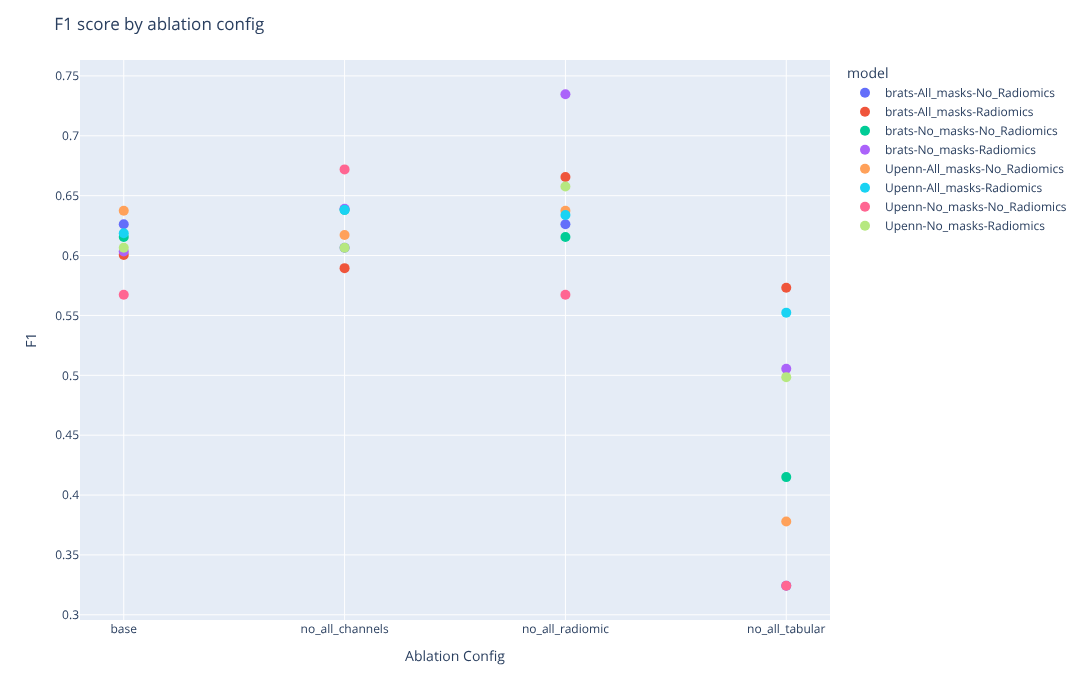
\includegraphics[width=\textwidth]{images/results_ablation.png}
    \end{column}
    \begin{column}{0.35\textwidth}
      \small
      \begin{itemize}
        \item Sin tabulares: \bad{notable caída de F1}. Modalidad más crítica
        \item Entrenar con radiómicos \good{mitiga} la falta de clínicos
        \item Predecir con radiómicos \bad{empeora}: el gate no los suprime
        \item Entrenar con dropout \good{mejora} en la mayoría de configuraciones
      \end{itemize}

    \end{column}
  \end{columns}
\end{frame}

% ============================================================
\begin{frame}{Ablación — BraTS, All Masks}
  \centering
  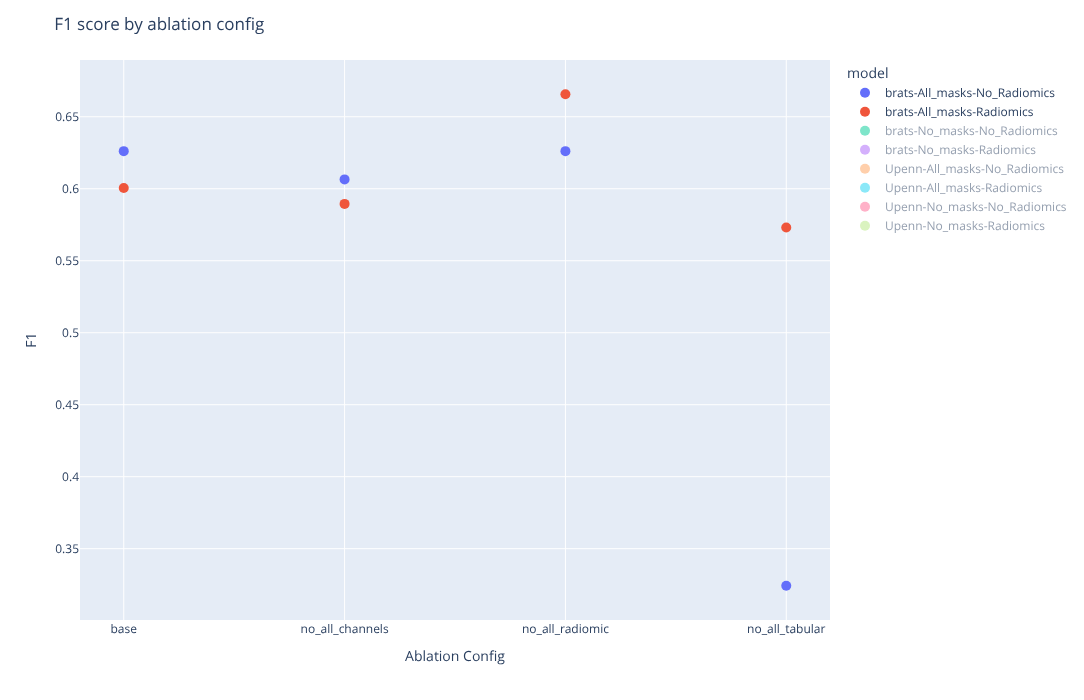
\includegraphics[width=0.8\textwidth]{images/ablation_brats_all_mask.png}
\end{frame}

\begin{frame}{Ablación — BraTS, Sin Máscaras}
  \centering
  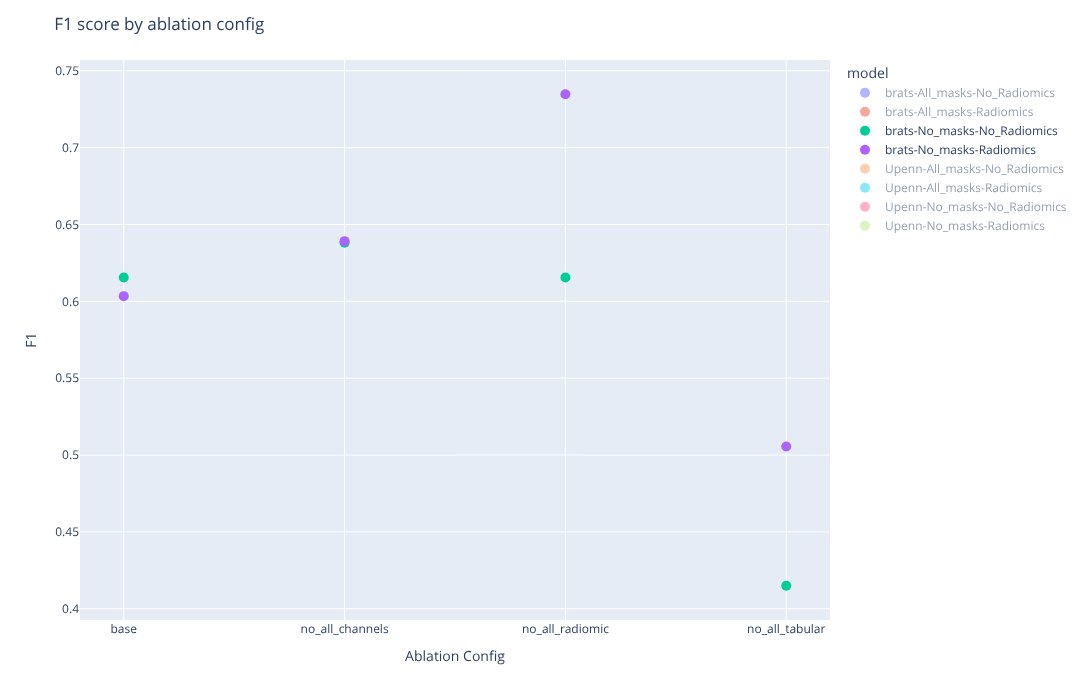
\includegraphics[width=0.8\textwidth]{images/ablation_brats_no_mask.png}
\end{frame}

\begin{frame}{Ablación — UPenn, All Masks}
  \centering
  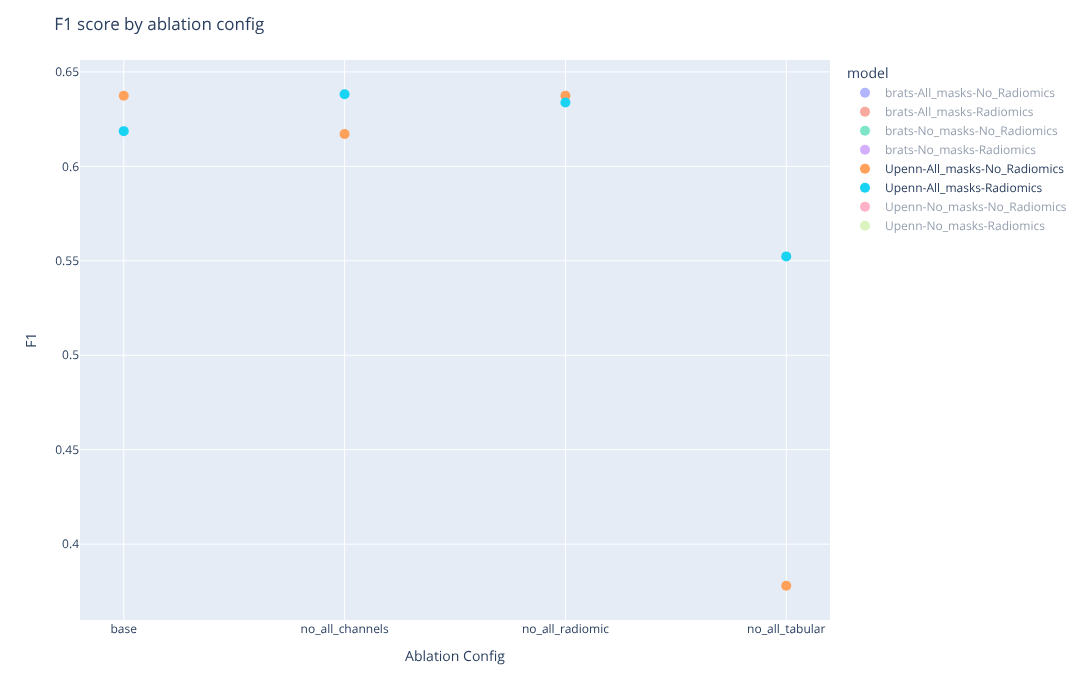
\includegraphics[width=0.8\textwidth]{images/ablation_upenn_all_mask.png}
\end{frame}

\begin{frame}{Ablación — UPenn, Sin Máscaras}
  \centering
  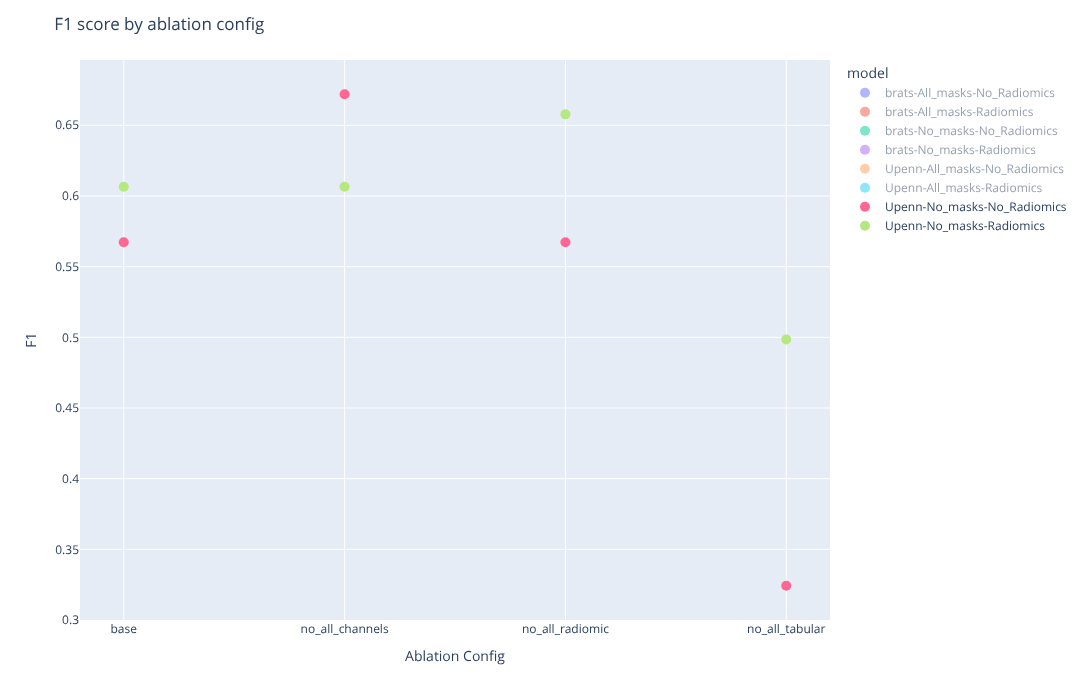
\includegraphics[width=0.8\textwidth]{images/ablation_upenn_no_mask.png}
\end{frame}

% ============================================================
\section{Conclusiones y trabajo futuro}

\begin{frame}{Conclusiones y trabajo futuro}
  \begin{columns}[T]
    \begin{column}{0.50\textwidth}
      \textbf{Conclusiones}
      \begin{enumerate}
        \item Modelo multimodal capaz de integrar MRI, datos clínicos y radiómicos de forma conjunta
        \item El modelo es robusto ante datos faltantes
        \item Se alcanza un F1 comparable al baseline pese a la mayor complejidad del problema
        \item El estudio ablacional confirma que los datos clínicos son la modalidad más crítica, y que los radiómicos mitigan su ausencia
      \end{enumerate}
    \end{column}

    \begin{column}{0.50\textwidth}
      \textbf{Trabajo futuro}
      \begin{enumerate}
        \item Explorar mecanismos de fusión que superen el \textit{gated fusion} actual
        \item Estudiar si el \textit{gate} aprende a suprimir los radiómicos en inferencia cuando no aportan información adicional a la imagen
        \item Ampliar la tarea a regresión de supervivencia
        \item Validar el modelo en centros externos para comprobar la generalización
      \end{enumerate}
    \end{column}
  \end{columns}

  \vspace{0.3cm}

  \begin{block}{Aporte principal}
      \footnotesize
    El principal aporte no es superar el estado del arte, sino demostrar que un único modelo puede tolerar ausencias arbitrarias de modalidades de forma aprendida, lo que lo hace directamente aplicable al entorno clínico real.
  \end{block}

\end{frame}

% ============================================================
\begin{frame}[plain]
  \centering
  \vspace{1.5cm}
  {\Huge\bfseries\color{darkgray}¿Preguntas?}

  \vspace{1.5cm}
  {\large Miquel Gómez Corral \quad $\cdot$ \quad Andrés Pacheco Millán}

  \vspace{0.4cm}
  {\small Máster en Inteligencia Artificial, Reconocimiento de Formas e Imagen Digital\\
  Universitat Politècnica de València}
\end{frame}

\end{document}